\documentclass[journal,12pt,twocolumn]{IEEEtran}

\usepackage{setspace}
\usepackage{gensymb}

\singlespacing


\usepackage[cmex10]{amsmath}

\usepackage{amsthm}

\usepackage{mathrsfs}
\usepackage{txfonts}
\usepackage{stfloats}
\usepackage{bm}
\usepackage{cite}
\usepackage{cases}
\usepackage{subfig}

\usepackage{longtable}
\usepackage{multirow}

\usepackage{enumitem}
\usepackage{mathtools}
\usepackage{steinmetz}
\usepackage{tikz}
\usepackage{circuitikz}
\usepackage{verbatim}
\usepackage{tfrupee}
\usepackage[breaklinks=true]{hyperref}

\usepackage{tkz-euclide}

\usetikzlibrary{calc,math}
\usepackage{listings}
    \usepackage{color}                                            %%
    \usepackage{array}                                            %%
    \usepackage{longtable}                                        %%
    \usepackage{calc}                                             %%
    \usepackage{multirow}                                         %%
    \usepackage{hhline}                                           %%
    \usepackage{ifthen}                                           %%
    \usepackage{lscape}     
\usepackage{multicol}
\usepackage{chngcntr}

\DeclareMathOperator*{\Res}{Res}

\renewcommand\thesection{\arabic{section}}
\renewcommand\thesubsection{\thesection.\arabic{subsection}}
\renewcommand\thesubsubsection{\thesubsection.\arabic{subsubsection}}

\renewcommand\thesectiondis{\arabic{section}}
\renewcommand\thesubsectiondis{\thesectiondis.\arabic{subsection}}
\renewcommand\thesubsubsectiondis{\thesubsectiondis.\arabic{subsubsection}}


\hyphenation{op-tical net-works semi-conduc-tor}
\def\inputGnumericTable{}                                 %%

\lstset{
%language=C,
frame=single, 
breaklines=true,
columns=fullflexible
}
\begin{document}


\newtheorem{theorem}{Theorem}[section]
\newtheorem{problem}{Problem}
\newtheorem{proposition}{Proposition}[section]
\newtheorem{lemma}{Lemma}[section]
\newtheorem{corollary}[theorem]{Corollary}
\newtheorem{example}{Example}[section]
\newtheorem{definition}[problem]{Definition}

\newcommand{\BEQA}{\begin{eqnarray}}
\newcommand{\EEQA}{\end{eqnarray}}
\newcommand{\define}{\stackrel{\triangle}{=}}
\bibliographystyle{IEEEtran}
\providecommand{\mbf}{\mathbf}
\providecommand{\pr}[1]{\ensuremath{\Pr\left(#1\right)}}
\providecommand{\qfunc}[1]{\ensuremath{Q\left(#1\right)}}
\providecommand{\sbrak}[1]{\ensuremath{{}\left[#1\right]}}
\providecommand{\lsbrak}[1]{\ensuremath{{}\left[#1\right.}}
\providecommand{\rsbrak}[1]{\ensuremath{{}\left.#1\right]}}
\providecommand{\brak}[1]{\ensuremath{\left(#1\right)}}
\providecommand{\lbrak}[1]{\ensuremath{\left(#1\right.}}
\providecommand{\rbrak}[1]{\ensuremath{\left.#1\right)}}
\providecommand{\cbrak}[1]{\ensuremath{\left\{#1\right\}}}
\providecommand{\lcbrak}[1]{\ensuremath{\left\{#1\right.}}
\providecommand{\rcbrak}[1]{\ensuremath{\left.#1\right\}}}
\theoremstyle{remark}
\newtheorem{rem}{Remark}
\newcommand{\sgn}{\mathop{\mathrm{sgn}}}
\providecommand{\abs}[1]{\left\vert#1\right\vert}
\providecommand{\res}[1]{\Res\displaylimits_{#1}} 
\providecommand{\norm}[1]{\left\lVert#1\right\rVert}
%\providecommand{\norm}[1]{\lVert#1\rVert}
\providecommand{\mtx}[1]{\mathbf{#1}}
\providecommand{\mean}[1]{E\left[ #1 \right]}
\providecommand{\fourier}{\overset{\mathcal{F}}{ \rightleftharpoons}}
%\providecommand{\hilbert}{\overset{\mathcal{H}}{ \rightleftharpoons}}
\providecommand{\system}{\overset{\mathcal{H}}{ \longleftrightarrow}}
	%\newcommand{\solution}[2]{\textbf{Solution:}{#1}}
\newcommand{\solution}{\noindent \textbf{Solution: }}
\newcommand{\cosec}{\,\text{cosec}\,}
\providecommand{\dec}[2]{\ensuremath{\overset{#1}{\underset{#2}{\gtrless}}}}
\newcommand{\myvec}[1]{\ensuremath{\begin{pmatrix}#1\end{pmatrix}}}
\newcommand{\mydet}[1]{\ensuremath{\begin{vmatrix}#1\end{vmatrix}}}
\numberwithin{equation}{subsection}
\makeatletter
\@addtoreset{figure}{problem}
\makeatother
\let\StandardTheFigure\thefigure
\let\vec\mathbf
\renewcommand{\thefigure}{\theproblem}
\def\putbox#1#2#3{\makebox[0in][l]{\makebox[#1][l]{}\raisebox{\baselineskip}[0in][0in]{\raisebox{#2}[0in][0in]{#3}}}}
     \def\rightbox#1{\makebox[0in][r]{#1}}
     \def\centbox#1{\makebox[0in]{#1}}
     \def\topbox#1{\raisebox{-\baselineskip}[0in][0in]{#1}}
     \def\midbox#1{\raisebox{-0.5\baselineskip}[0in][0in]{#1}}
\vspace{3cm}
\title{EE5600 Assignment 4}
\author{Abhishek Thakur}
\maketitle
\newpage
\bigskip
\renewcommand{\thefigure}{\theenumi}
\renewcommand{\thetable}{\theenumi}
\newcommand\hlight[1]{\tikz[overlay, remember picture,baseline=-\the\dimexpr\fontdimen22\textfont2\relax]\node[rectangle,fill=blue!50,rounded corners,fill opacity = 0.2,draw,thick,text opacity =1] {$#1$};}
\begin{abstract}
This document contains the solution of Quadratic equation using gradient descent.
\end{abstract}
Download latex and python codes from 
\begin{lstlisting}
https://github.com/abhishekt711/EE5600/tree/master/Assignment_4
\end{lstlisting}
%
\section{Problem}
Find the maximum and minimum values, if any, of the follwing function given by\\
    $f(x)=(2x-1)^2+3$
\section{Explanation}
Given Equation can be written as:
\begin{align}
    f(x)=(2x-1)^2+3=4x^2-4x+4
\end{align}
   A function is said to be convex if following inequality is true:
    \begin{align}
        \lambda f(x_1)+(1-\lambda) f(x_2) \geq f(\lambda x_1+(1-\lambda) x_2)
    \end{align}
    and for $\lambda \in [0,1]$
\begin{align}
&\lambda(4x_1^2-4x_1+4)+(1-\lambda)((4x_2^2-4x_2+4) \geq \nonumber \\ 
&4(\lambda x_1 +(1-\lambda )x_2)^2-4(\lambda x_1 +(1-\lambda )x_2)+4\\
&x_1^2(4\lambda-4\lambda^2)+x_2^2(4\lambda-4\lambda^2)-2x_1x_2(4\lambda-4\lambda^2) \geq 0\\
&4\lambda(1-\lambda)(x_1-x_2)^2 \geq 0
\end{align}
The above inequality is always true for all values from the domain. Hence the given function f(x) is convex.
%\begin{align}
%	\vec{x}^T\myvec{4&0\\0&0}\vec{x}  + \myvec{-4&0}\vec{x} +4 = 0
%\end{align}


    Using gradient descent method,
    \begin{align}
    x_1=x_0-\mu\frac{df(x)}{dx} \label{eq2}
    \end{align}
    Here, $\mu$ is learning rate.\\
    \begin{align}
    \frac{df(x)}{dx}=8x-4
\end{align}
    Taking $\mu=0.1$, $x_0=2$ and substiuting in equation \ref{eq2} . After 4 iteration, the value of $x$ where minima occurs is:
    \begin{align}
    x=0.50048
    \end{align}
After each iteration starting from x=2,when we come leftward on x-axis the slope increases i.e, slope becoming less negative. Thus, it is a convex function.\\
At maxima / minima slope of $f(x)$ will be zero.
\begin{align}
    \frac{df(x)}{dx}=0\\
	\implies 8x-4=0\\
    \therefore x=0.5
\end{align}
Now, to know whether x=0.5 is the point of maxima or minima, we need to calculate $f''(x)$.
\begin{align}
    \frac{d''f(x)}{dx}=8
\end{align}
$\because   \frac{d''f(x)}{dx}>0$, therefore,  we can conclude that x=0.5 is the point of minima.\\
At $f(x)$ at x=0.5,
\begin{align}
    f(0.5)=3
\end{align}
	\begin{figure}[!ht]
	\centering
	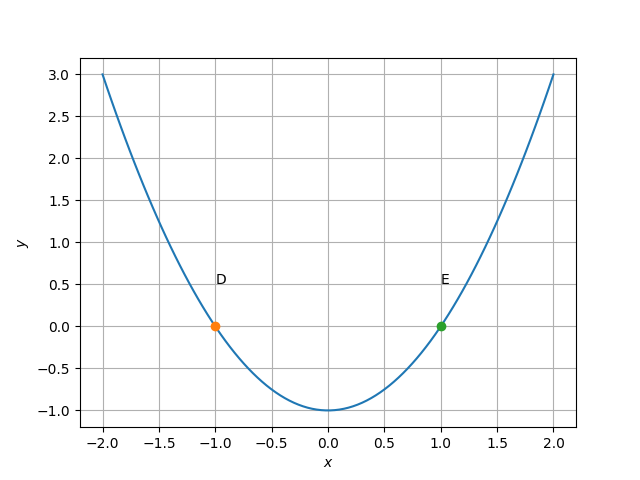
\includegraphics[width=\columnwidth]{Figure_1.png}
	\caption{Plot of the given polynomial}
	\label{fig:5.1}	
	\end{figure}
	\begin{lstlisting}
	./codes/Assignment_4.py
	\end{lstlisting}
The following python code computes the minimum value of the given polynomial as plotted in Fig. \ref{fig:5.1}.\\
Hence, The minimum value of $f(x)$ at $x=0.5$ is 3.
\end{document}